% !TEX root = ../notes.tex

% ================ Statistics ==============
\section{Statistics on the Data}

When we explore and analyze data, it would be great if we only had to look at some statistics numbers and make automatically a conclusion about them. Sadly, it's not the case. At all.
% ================  Famous mistakes ==============
\subsection{Examples of famous mistakes due to statistics}

%=================== Anscombe's quartet ===================
\subsubsection{Anscombe's quartet: Sensivity of outliers \& Robust statistics}

The FIG \ref{pic:anscombe} show four different data distribution that present, despite all of that, the same means on $x$ and $y$, the same variance on $x$ and $y$, and, thus, the same linear regression function. This is due to the statistics used to define them. 

\begin{itemize}
    \item Min, Max, Mean, Standard Deviation (Std) and Range are sensitive to outliers and then are \textbf{not robust statistics}.
    \item Median, quartils, (and others) are not sensitive and then are said to be \textbf{robust statistics}. 
\end{itemize}



\begin{figure}[h]%---------------FIG--------------
 \centering
 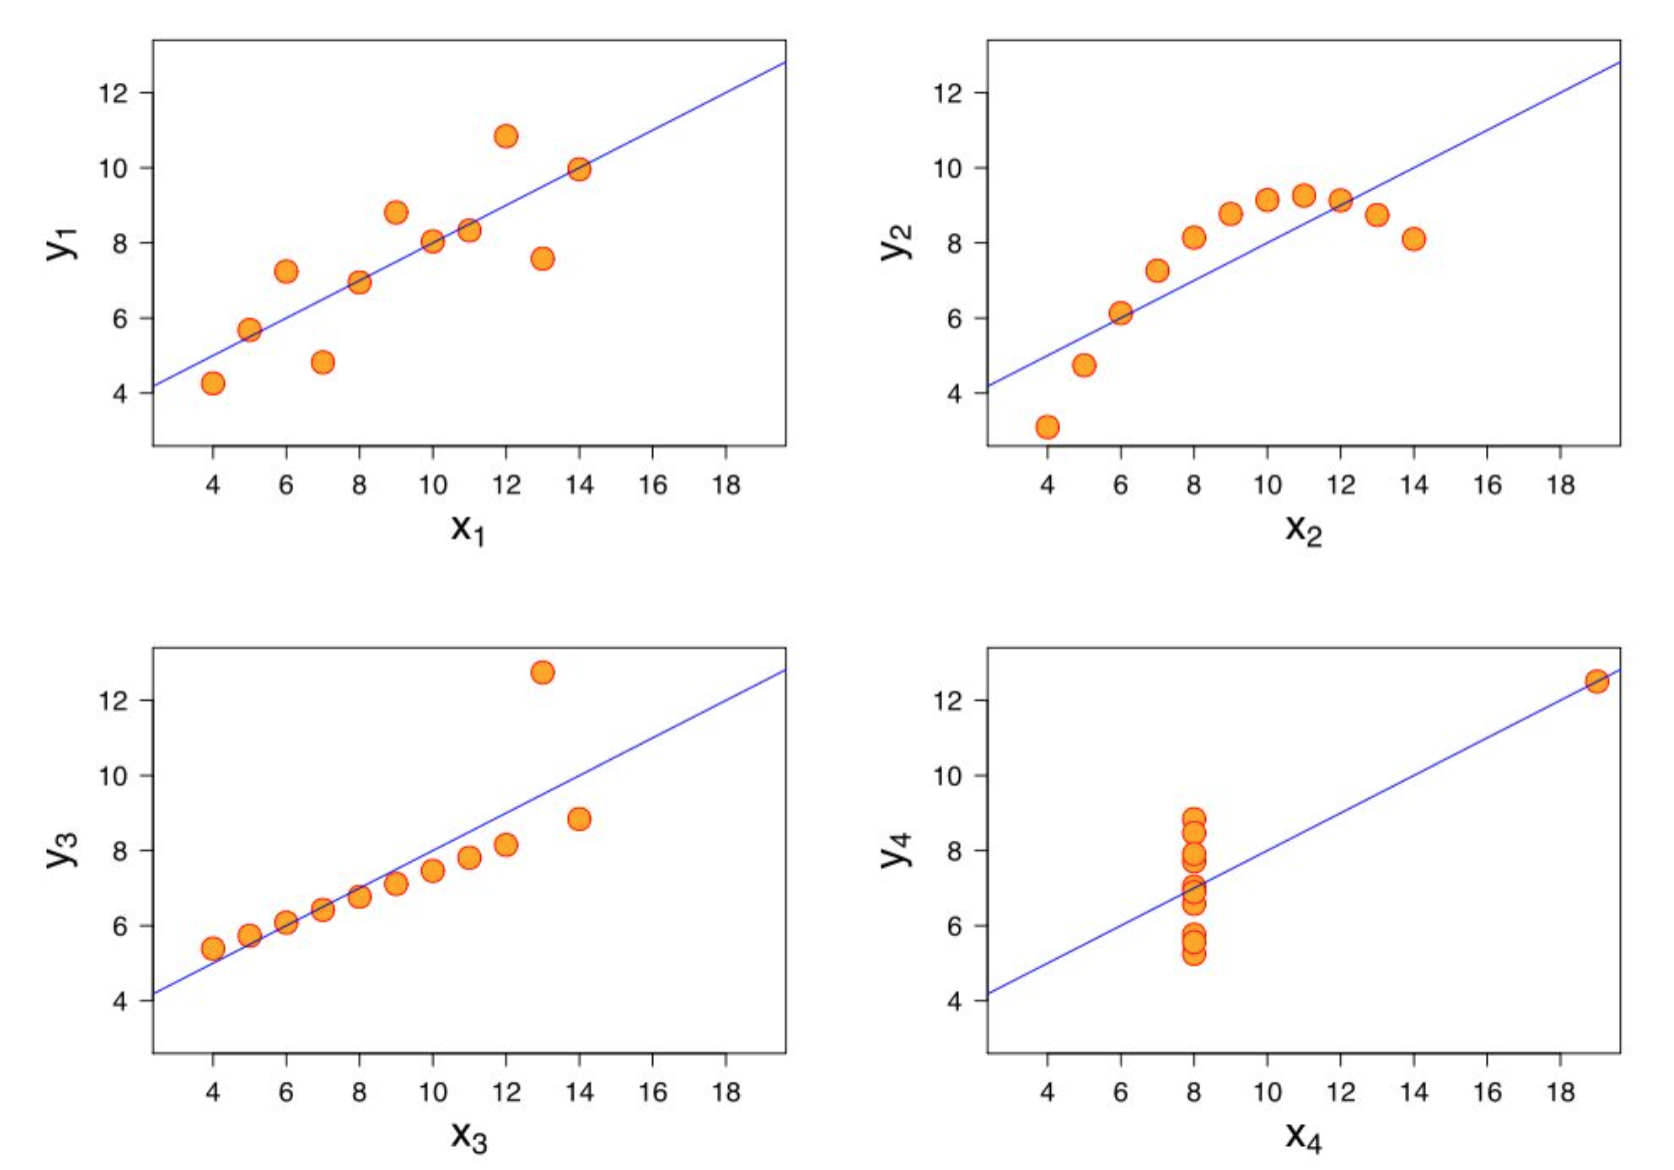
\includegraphics[width=10cm]{./img/05/anscombe}
 \caption{\label{pic:anscombe} Anscombe's quartet}
\end{figure}

%================ Simpson paradox =================
\subsubsection{Simpson's paradox: aggregation of data}

\textbf{Certain tendencies can appear, disappear or even reverse themselves when aggregating the data!} This was the case when media started blaming Berkey of being unfair with women applications (looking at left table of FIG \ref{pic:Berkley}). After further investigation (and de-aggregation of the data), it appeared that at the opposite... Berkeley was unfair with men! (Right table of the same FIG).

This paradox comes from the fact that women (according to these tables) tended to apply for more competitive departments, with lower rates of admission. \textbf{When aggregating the data, we lost this subtlety and then draw a wrong conclusion.} 

Simpson's paradox can appear in a lot of cases and can be very hard to detect. The \href{https://en.wikipedia.org/wiki/Simpsons_paradox}{wikipedia page of Simpson's paradox} describes a lot of examples and, for the ones interested, a great book relates lots of statistical errors that drove to miscarriages of justice: \href{https://books.google.ch/books/about/Math_on_Trial.html?id=PFAIb6FTgY4C&source=kp_cover&redir_esc=y&hl=fr}{Leila Schneps and Coralie Colmez, Math on Trial: How Numbers Get Used and Abused in the Courtroom} 

\begin{figure}[h]%---------------FIG--------------
 \centering
 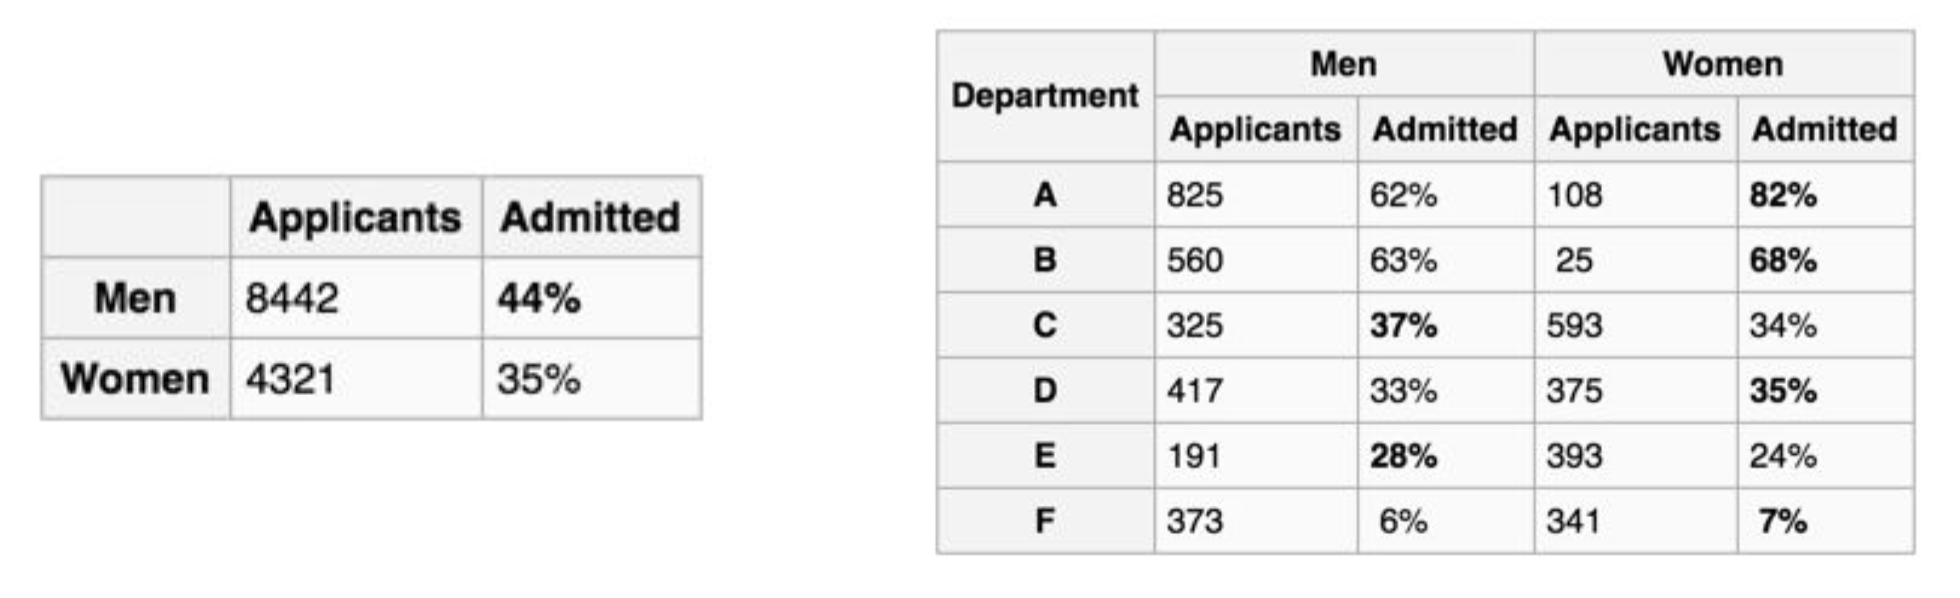
\includegraphics[width=10cm]{./img/05/Berkeley}
 \caption{\label{pic:Berkley}Berkley admission tables of 1973}
\end{figure}

% ================ Basic stats ==============
\subsection{Refresh of basic statistics concept}

\begin{itemize}
	\item {\bf Probabilities}: mathematical theory that describes uncertainty. \\
	\item {\bf Statistics}: Set of techniques for extracting useful info from data
\end{itemize}

\begin{framed}
{\it {\bf Probability and Statistics} are related areas of mathematics which concern themselves with analyzing the relative frequency of events. Still, there are fundamental differences in the way they see the world:\\
\textbf{Probability deals with predicting the likelihood of future events}, while \textbf{statistics involve the analysis of the frequency of past events}. \\  
Probability is primarily a theoretical branch of mathematics, which studies the consequences of mathematical definitions. Statistics is primarily an applied branch of mathematics, which tries to make sense of observations in the real world.}
\signed{\href{http://www3.cs.stonybrook.edu/~skiena/jaialai/excerpts/node12.html}{Steven S. Skiena, "Calculated Bets", Cambridge University Press, 2001}}
\end{framed}

% ================ Bayes Theorem ==============
\subsubsection{Bayes Theorem}
The theorem express the very intuitive statement that:

{\it The probability of observing event A and B is the probability of observing B multiplied by the probability of observing A knowing that B occurred.}

Mathematically it's expressed as: 
\be
P(A\vert B)P(B)=P(A\cap B)=P(B\vert A)P(A)
\ee
Or equivalently
\be
P(A|B)={\frac  {P(B|A)P(A)}{P(B)}}
\ee

More about Bayes Theorem on \href{https://en.wikipedia.org/wiki/Bayes_theorem}{wikipedia}.

% ================ Random Variables ==============
\subsubsection{Random Variables}
A \textbf{random variable} is a quantity that can take various values, each one associated with a probability of apparitions. The some of these probabilities will always be 1.
\be
X\colon \Omega \to E
\ee

$\Omega$ being a probability space and $E$ a measurable space (usually $E = \mathbb{R}$).

Any random variable can be described by its \href{https://en.wikipedia.org/wiki/Cumulative_distribution_function}{cumulative distribution function}, which describes the probability that the random variable will be less than or equal to a certain value.

Two \textbf{independent variables} are defined as
\be
{\mathbb  {P}}(A\cap B)={\mathbb  {P}}(A)\cdot {\mathbb  {P}}(B).
\ee
or equivalently (by Bayes Theorem)
\be
\label{indep}
{\mathbb  {P}}(A\mid B) =  {\mathbb  {P}}(A)
\ee

More about Bayes Theorem on \href{https://en.wikipedia.org/wiki/Random_variable}{wikipedia}.

% ================ Law of Large Number ==============
\subsubsection{Law of Large Numbers}

The Law of Large Numbers links, in some way, the probability to the statistics. It's, again, a very intuitive statement, even if not so easy to prove (as always in mathematics).

\begin{framed}
In probability theory, the\textbf{ law of large numbers} (LLN) is a theorem that describes the result of performing the same experiment a large number of times. According to the law, \textbf{the average of the results obtained from a large number of trials should be close to the expected value}, and will tend to become closer as more trials are performed.
\signed{\href{https://en.wikipedia.org/wiki/Law_of_large_numbers}{Wikipedia}}
\end{framed}

A common mistake is to deduce that, in the case of playing heads or tails for example, observing a lot of time \textbf{heads} increase the probability of observing \textbf{tails}. This is absolutely wrong. The variables are perfectly independent and, according to Eq \ref{indep}, the probability stays exactly 50\%. This is the perfect example of confusing probabilities with statistics.

% ================ CLT ==============
\subsubsection{Central Limit Theorem}

\textbf{Central Limit Theorem} states that the mean of independent and identically-distributed random variables will converge to \textbf{Gaussian Distribution} (Normal Distribution).

% ================ CLT ==============
\subsection{Most common distributions}

\begin{itemize}
	\item \textbf{Gaussian Distribution} (fig \ref{gauss}) results from independent and identically-distributed variables 
	$f(x\;|\;\mu ,\sigma ^{2})={\frac {1}{\sqrt {2\sigma ^{2}\pi }}}\;e^{-{\frac {(x-\mu )^{2}}{2\sigma ^{2}}}}$
	\href{https://en.wikipedia.org/wiki/Gaussian_distribution}{More on wikipedia}
	
	\item \textbf{Poisson Distribution} (fig \ref{poisson}) describe the observation of events happening in a delimited time-laps. E.g: an event happens in average 4 times each 10 minutes ($\lambda = 4$). What's the probability that it appears after only 3 times in this same interval ($k = 3$)? $p(k) = \frac{\lambda ^k}{k!}e^{-\lambda}$ \href{https://en.wikipedia.org/wiki/Poisson_distribution}{More on wikipedia}

	\item \textbf{Exponential Distribution} (fig \ref{exp}) describes the time between two events in a Poisson process. $P(x) = \lambda e^{- \lambda x}$ \href{https://en.wikipedia.org/wiki/Exponential_distribution}{More on wikipedia}
	
	\item \textbf{Binomial Distribution} (fig \ref{binomial}) describes the discrete distribution on success in a yes/no experiment. (E.g. coin tossing or any win/lose game). $f(k;n,p)=\Pr(X=k)={\binom {n}{k}}p^{k}(1-p)^{n-k}$ \href{https://en.wikipedia.org/wiki/Binomial_distribution}{More on wikipedia}
	
	\item \textbf{Multinomial Distribution} generalizes Binomial law. \href{https://en.wikipedia.org/wiki/Multinomial_distribution}{More on wikipedia}
	
	\item \textbf{Zipf Distribution} is an empirical discret description of word frequency in a text. \href{https://en.wikipedia.org/wiki/Zipfs_law}{More on wikipedia}
	
	\item \textbf{Pareto Distribution} is the equivalent of Zipf in a continuous space. It allows, amongst other things, to give a theoretical base of the "80-20 principle" (20\% of the causes produce 80\% of the effects). \href{https://en.wikipedia.org/wiki/Pareto_distribution}{More on wikipedia}
	
	\item \textbf{Yule-Simon distribution} describes discret frequencies of term too. \href{https://en.wikipedia.org/wiki/Yule?Simon_distribution}{More on wikipedia}
\end{itemize}

{\bf \color{red}  You should understand the distribution of your data before applying a model!}

\begin{figure}[H] %----------- SubGraph ---------------------
\centerline{
\subfigure[Probability density function] {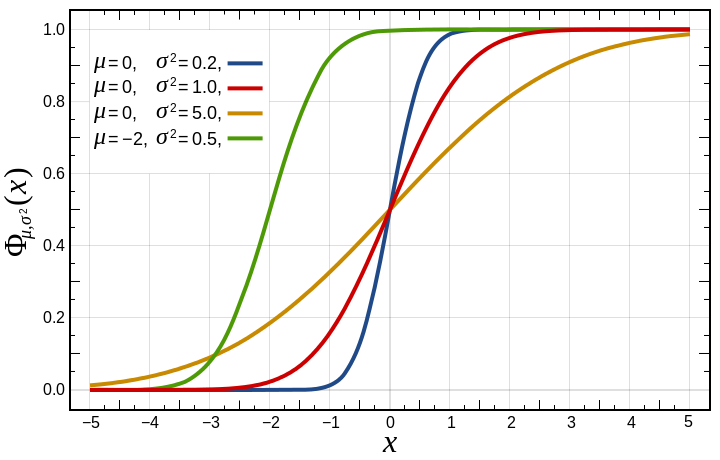
\includegraphics[width=5.5cm]{img/05/gauss_density}}
\subfigure[Cumulative distribution function] {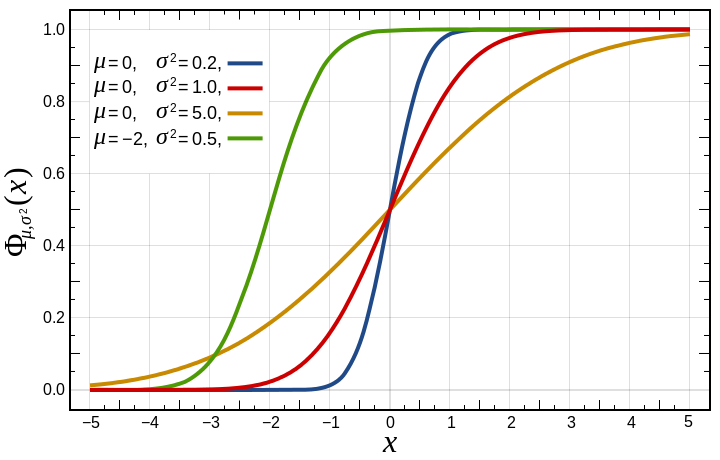
\includegraphics[width=5.5cm]{img/05/gauss_cumul}} 
}
\caption{\label{gauss} 
Gaussian distribution 
} 
\end{figure}
\begin{figure}[H] %----------- SubGraph ---------------------
\centerline{
\subfigure[Probability density function] {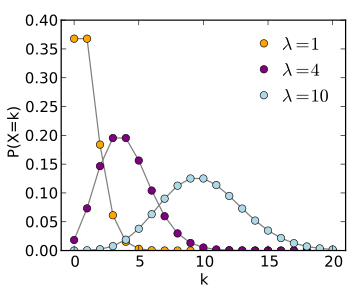
\includegraphics[width=5.5cm]{img/05/Poisson_pmf}}
\subfigure[Cumulative distribution function] {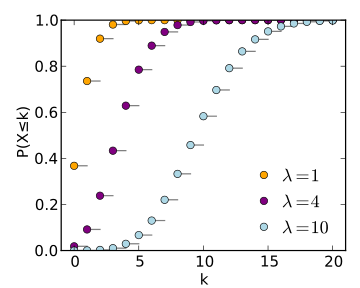
\includegraphics[width=5.5cm]{img/05/Poisson_cdf}} 
}
\caption{\label{poisson} 
Poisson distribution 
}
\end{figure}
\begin{figure}[H] %----------- SubGraph ---------------------
\centerline{
\subfigure[Probability density function] {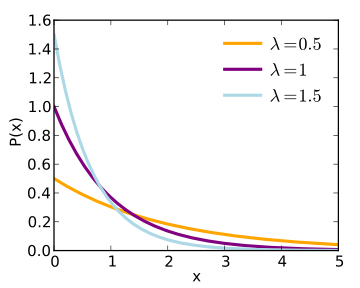
\includegraphics[width=5.5cm]{img/05/exp_pmf}}
\subfigure[Cumulative distribution function] {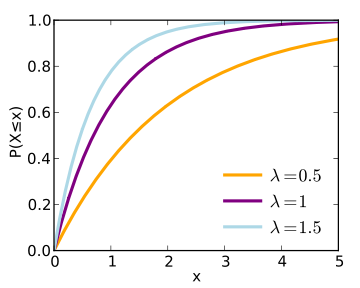
\includegraphics[width=5.5cm]{img/05/exp_cdf}} 
}
\caption{\label{exp} 
Exponential distribution 
} 
\end{figure}
\begin{figure}[H] %----------- SubGraph ---------------------
\centerline{
\subfigure[Probability density function] {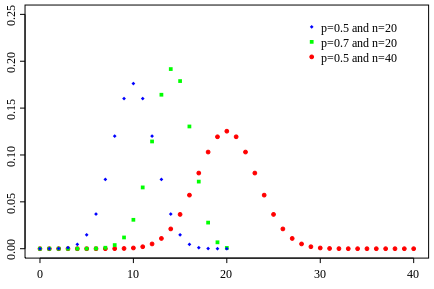
\includegraphics[width=5.5cm]{img/05/binomial_pmf}}
\subfigure[Cumulative distribution function] {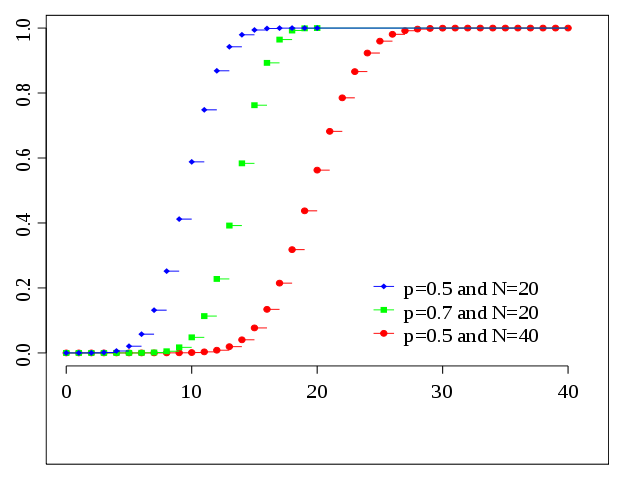
\includegraphics[width=5.5cm]{img/05/binomial_cdf}} 
}
\caption{\label{binomial} 
Binomial distribution 
} 
\end{figure}



% ================ Measurement ==============
\subsection{Measurement on Samples}

In practice, we (almost) never analyse the entire population. We always work on a subset of it called \textbf{sample}. The \textbf{variance} is the variation between elements of our sample, that we hope to be the same as the population. The \textbf{biases} is the systematic variation between the entire population and the sample we chose.

When randomly select elements of the population to be part of the sample, we have a great chance that the bias is small (i.e. that the distribution of the sample corresponds to the distribution of the population). But do not forget that there is a probability (even if a small one) to select elements that \textbf{biased our measures}! This probability can even increase when you clean the data, if you don't do it wisely.

A stupid example could be a study on population education in which, during the cleaning, you remove the answers containing misspelling. Uneducated people are more likely to commit misspelling so, removing them, you artificially biais the sample.

% ================ Test Statistic ==============
\subsection{Test Statistic}

(The only good and easy-to-understand explanation about test statistics I ever found is available on \href{http://hamelg.blogspot.ch/2015/11/python-for-data-analysis-part-24.html?view=flipcard}{hamelg.blogspot})

The idea behind test statistics is \textbf{instead of proving that our assumption is true, let's calculate the probability that our observations occur by chance (null hypothesis or $H_0$). If this probability is very low, then there is a good chance that our hypothesis is true!}

The probability that this happens by chance is called $pvalue$ and we usually consider that if $pvalue \leq 0.05$ our hypothesis is true ($pvalue \leq 0.01$ in some strict cases).

% ================ Test Statistic ==============
\subsubsection{Example with t-test}

Let's take the example on FIG \ref{pic:ttest}. The \textbf{Null Hypothesis} $H_0$ represents the distribution of observation we can do, assuming there is no correlation between the values we measured. The \textbf{Alternative} is $H_A$, our hypothesis which states that, at the opposite, there is correlations.
\begin{itemize}
	\item If the observation we test is $x=3$, there is \textbf{less than 5\% probabilities that it was produced by $H_0$} ($pvalue \leq 0.05$). Our hypothesis $H_A$ is considered true.

	\item If the observation we test is $x=0$, there are \textbf{more than 5\% probabilities that it was produced by $H_0$} (more or less 40\%). Our hypothesis $H_A$ is considered false.
\end{itemize}

{\color{red} An important thing to notice is that \textbf{it does not provide the truth on statistic}, it only provides information about how likely is the null hypothesis! Let's look back to the example}

\begin{itemize}
	\item The $x=3$ observation \textbf{could have been produced by the red area}, meaning that it's part of the small 5\% chance of being produced by the $H_0$. The test will say that our hypothesis is true, which will be a \textbf{false positive}.

	\item The $x=0$ observation \textbf{could have been produced by the blue area}, meaning that even it $H_0$ have great chance to produce it, it was in fact produced by $H_A$.  The test will say that our hypothesis is false, which will be a \textbf{false negative}.
\end{itemize}

\begin{figure}[h]%---------------FIG--------------
 \centering
 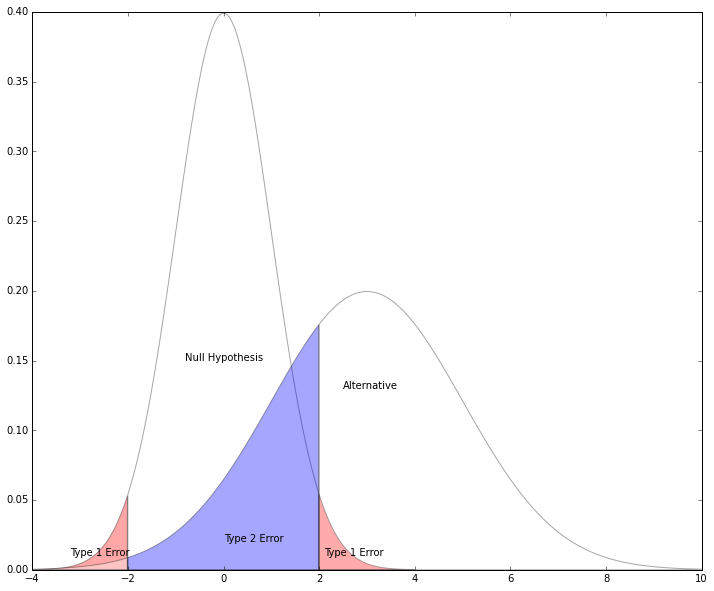
\includegraphics[width=10cm]{./img/05/t-test}
 \caption{\label{pic:ttest} T-Test example}
\end{figure}

% ================ Test Statistic ==============
\subsubsection{Choose the right test}

A lot of tests exist and we must choose wisely which one to use, according to data and hypothesis characteristics. FIG \ref{pic:testtree} show a decision tree helping to choose the test which suits best our situation.

\begin{itemize}
 \item Question ? 
 \item Data type ?
 \item Sample size
 \item Variance known? 
 \item Variance of several groups equals?
 \item ...
\end{itemize}

\begin{figure}[h]%---------------FIG--------------
 \centering
 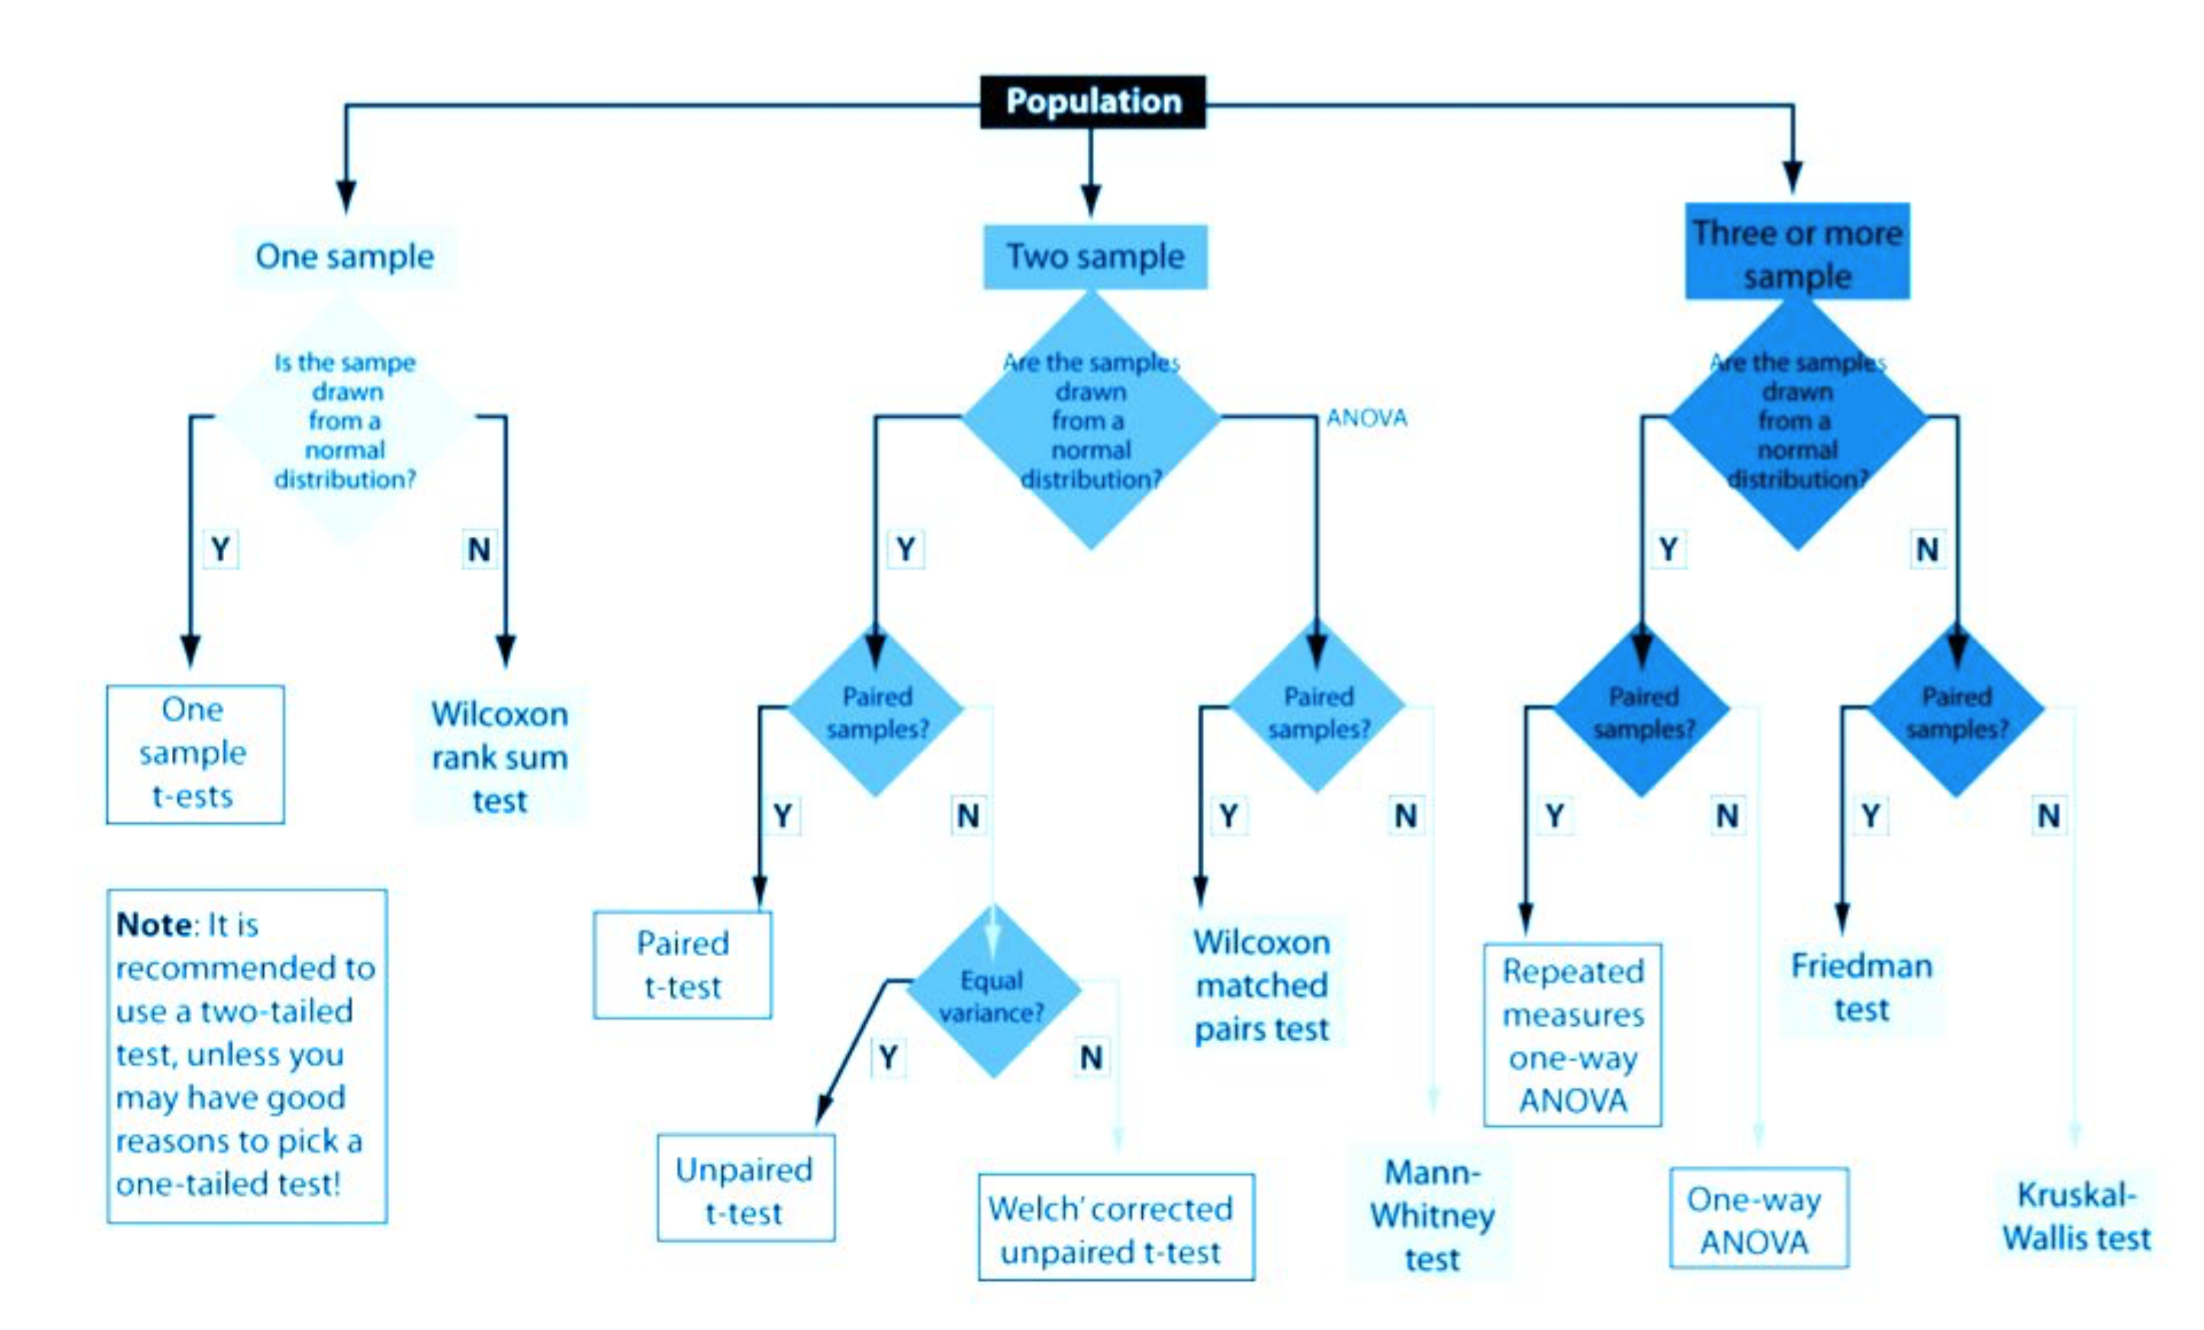
\includegraphics[width=15cm]{./img/05/choose_test}
 \caption{\label{pic:testtree} Statistical test decision tree}
\end{figure}


% ============================================
\subsubsection{Family-wise Error}

Following this simple math equation, we can figure out that the more experiment we do to test the hypothesis, the more likely we are to find that one of them are spuriously right! This is because the reverse point of view of the test. We are testing the fact that $H_0$ is unlikely, not directly that $H_A$ is likely. 

\begin{equation} \label{eq1}
\begin{split}
P(false \: positive) &= \alpha = 0.05 \\ 
P(true \: positive) &= 1 - \alpha = 0-95 \\
P(true \: positive \: on \: each \: experiment) &= (1 - \alpha)^k \\
P(at \: least \: on \: false \: positive \: on \: one \: experiment) &= 1 - (1 - \alpha)^k
\end{split}
\end{equation}

To counter that, two possible correction exists
\begin{itemize}
  \item Bonferroni correction : $\alpha_c = \frac{\alpha}{k}$ 
  \item Sidak correction: $\alpha_c = 1- (1 - \alpha)^{1/k} $
\end{itemize}


% ============================================
\subsubsection{Non-Parametric tests}

All the tests so fare assume that the data are {\bf normally distributed} and that the samples are {\bf independent of each other and all have the same distribution.} (IID) They may be inaccurate if those assumptions are not met. Therefore, make sure the data satisfy the assumptions of the test we're using. Watch out for:
\begin{itemize}
 \item \textbf{Outliers} will corrupt many tests that use variance estimates.
 \item \textbf{Correlated values as samples}, e.g. if you repeated measurements on the same subjective
 \item \textbf{Skewed (bias) distributions} give invalid results.
\end{itemize}

Some tests make no assumptions and thus can be used on very general cases: \textbf{K-S test}, \textbf{Permutation test} and \textbf{Bootstrap confidence interval}.


%================================================
\subsubsection{K-S test}
K-S (Kolmogorov-Smirnov) test is a very useful test for checking whether two (continuous or discrete) distributions are the same. 
\begin{itemize}
 \item In the {\bf one-sided test}, an observed distribution (e.g. some observed values or a histogram) is compared against a reference distribution (e.g., power-law).
 \item In the {\bf two-sided test}, two observed distributions are compared.
 \item The K-S statistic is just the {\bf max distance between the CDFs} (Cumulative Distribution Function) of the two distributions.
 \item The K-S test can be used to test {\bf whether a data sample has  a normal distribution} or not.
 \item Thus it can be used as a sanity check for any common parametric test (which assumes normally distributed data).
 \item It can also be used to compared distributions of data values in large data pipeline: {\bf Most errors will distort the distribution of a data parameter and a K-S test can detect this.}
\end{itemize}
This test is expensive! Check for more information on the \href{https://en.wikipedia.org/wiki/Kolmogorov?Smirnov_test}{wikipedia page}.
